\documentclass[calculator,steamtables,refrigeranttables]{exam}
% The full list of class options are
% calculator : Allows approved calculator use.
% datasheet : Adds a note that data sheet are attached to the exam.
% handbook : Allows the use of the engineering handbook.
% resit : Adds the resit markings to the paper.
% sample : Adds conspicuous SAMPLE markings to the paper
% solutions : Uses the contents of \solution commands (and \solmarks) to generate a solution file
% steam and refrigerant tables

\coursecode{EG3521}%
\coursetitle{Engineering Thermodynamics}%
\examtime{00.00--00.00}%
\examdate{00}{05}{2014}%
\examformat{Candidates must attempt \textit{all} questions.}

\newcommand{\frc}{\displaystyle\frac}

\begin{document}

%%%
%%% Question 01 
%%%
\begin{question} %\vspace{-2\baselineskip}
A steam power plant operates with coupled regenerative and reheat Rankine cycle with 2 connected turbines as shown in Fig. \ref{exam_mod02_rankinecycle}.  Primary steam is supplied by the boiler at 120 bar and 565$^{\text{o}}$C. Conditions for water/steam flows are described in Table \ref{exam1_table1}. 

\begin{figure}[h]
\begin{center}
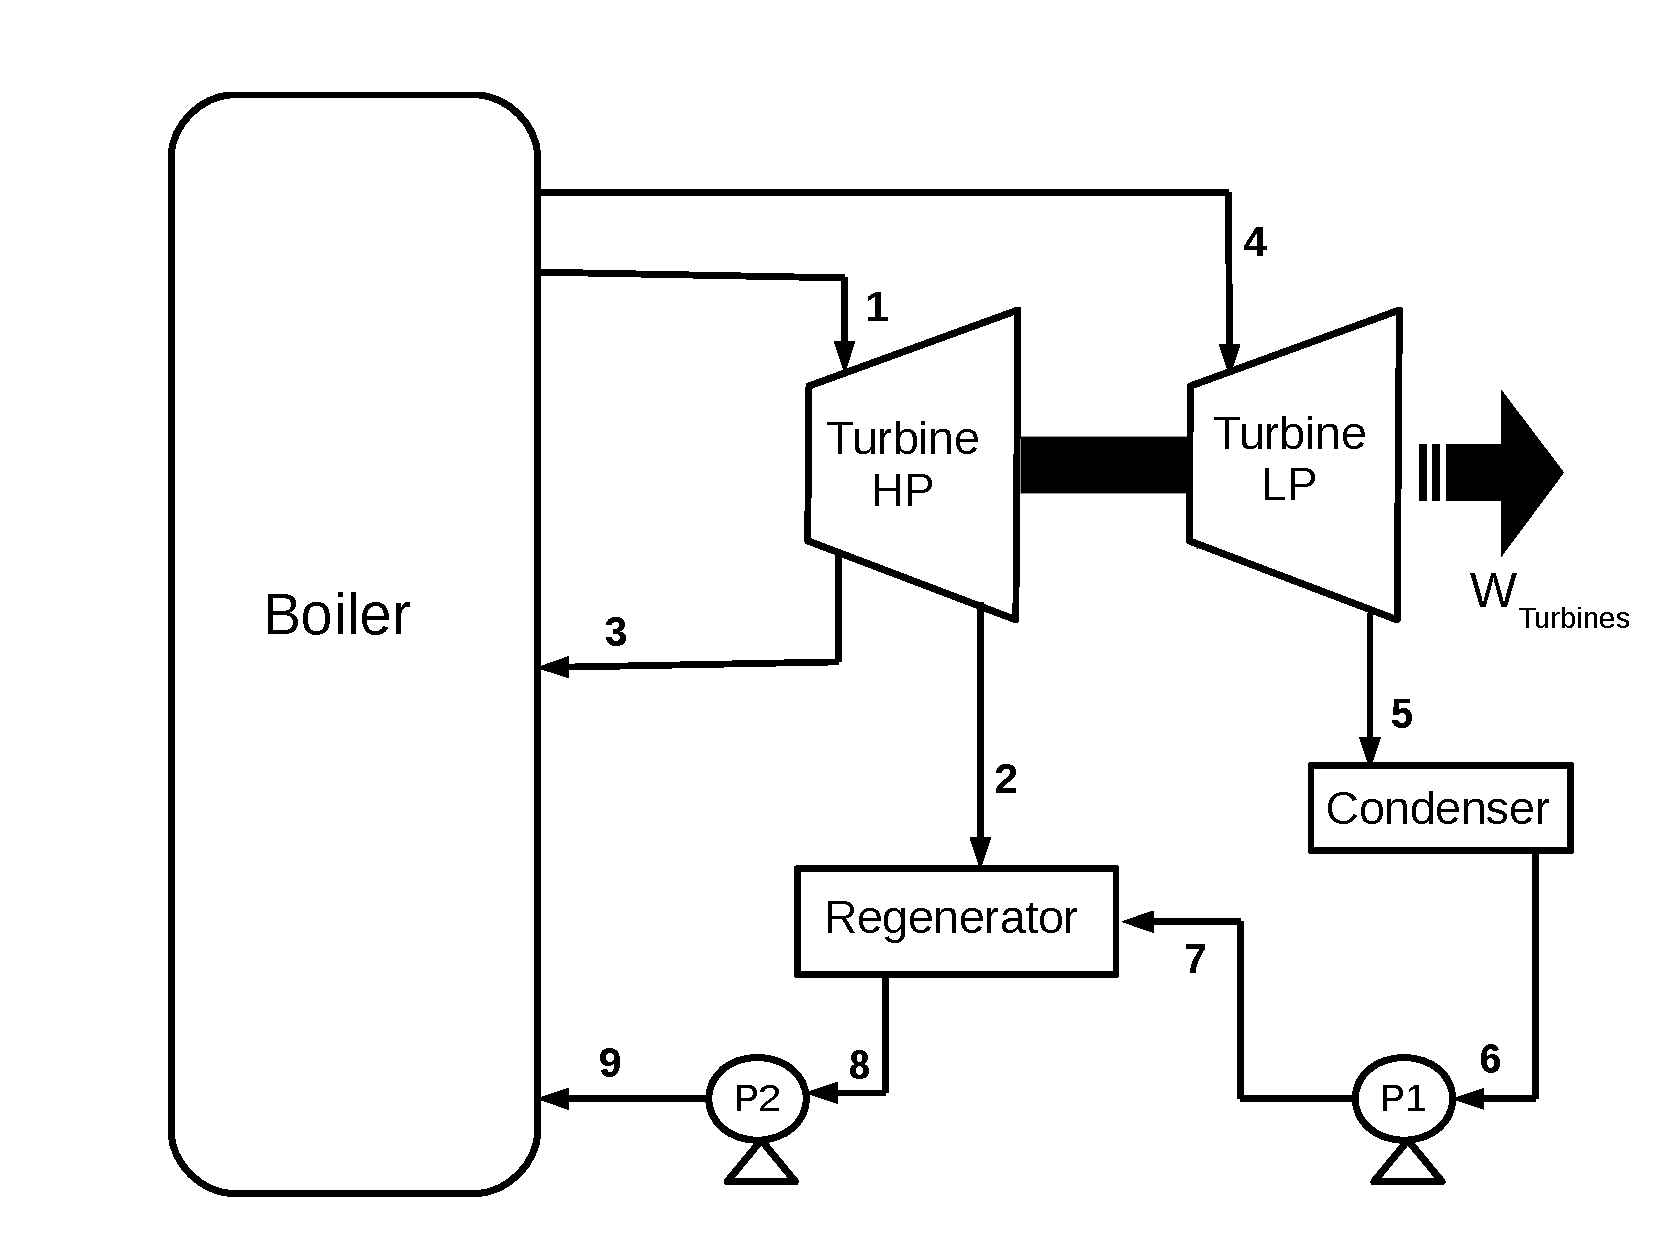
\includegraphics[width=15.cm,clip]{./Pics/Exam_Reheat_Regenerative_Rankine_Cycle}
\caption{ Reheat and regenerative Rankine cycle with 2 turbines.}
\label{exam_mod02_rankinecycle}
\end{center}
\end{figure}

\begin{table}[h]
\begin{center}
\begin{tabular} {||c | c c c c c c || }
\hline\hline
{\bf Stage} & {\bf P}    & {\bf T}        & {\bf State}    & {\bf H}             & {\bf S}                  & {\bf Steam}\\
            & {\bf (bar)}& {\bf ($^{o}$C)} &               & {\bf (kJ.kg$^{-1}$)} & {\bf (kJ.(kg.K)$^{-1}$)}  & {\bf Quality}\\
\hline\hline
 {\bf 1 }   & 120        & 565            &   {\bf (a)}    & {\bf (b)}           & {\bf (c)}                & --          \\
 {\bf 2 }   & 3          &  --            &   wet vapour   & {\bf (d)}           &   --                     & {\bf (e)}   \\
 {\bf 3 }   & 3          & 250            &   --           & --                  & --                       & --           \\
 {\bf 4 }   & 3          & 475            &   --           & --                  & --                       & --            \\
 {\bf 5 }   & 0.06       & --             &   wet vapour   & {\bf (f)}           & --                       & {\bf (g)}     \\
 {\bf 6 }   & --         & --             &   sat.liquid   & {\bf (h)}           & --                       & -- \\
 {\bf 7 }   & 3          & --             &   --           & {\bf (i)}           & --                       & --     \\
 {\bf 8 }   & 3          & --             &   --           & --                  & --                       & --           \\
 {\bf 9 }   & 120        & --             &   --           & {\bf (j)}           &  --                      & -- \\
\hline\hline
\end{tabular}
\end{center}
\caption{Thermodynamic table of the reheat and regenerative Rankine cycle (Question 1).}
\label{exam1_table1}
\end{table}


\begin{enumerate}[(a)]
\item In Table \ref{exam1_table1}, determine {\it (a)-(j)}. {\bf [10 Marks]}
%
\item Calculate the fraction (as $\%$) of steam supplied to the low-pressure (LP) turbine. {\bf [2 Marks]}
%
\item Determine the heat supplied by the boiler. {\bf [2 Marks]}
%
\item Determine the thermal efficiency of the cycle, {\bf [6 Marks]}
\begin{displaymath}
\eta=\frc{W_{Total}}{Q_{Boiler}} = \frc{\sum W_{\text{Turbines}} - \sum W_{\text{Pumps}}}{Q_{Boiler}}
\end{displaymath} 
%
\end{enumerate}

To solve this problem, you should assume that the saturated liquid streams are incompressible, and therefore $dH = VdP$ (where $H$, $V$ and $P$ are enthalpy, volume and pressure, respectively). Quality of the steam is expressed as
\begin{displaymath}
x_{j} = \frc{\Psi_{j}-\Psi_{f}}{\Psi_{g}-\Psi_{f}}\;\;\;\text{with }\Psi=\left\{H,S\right\}
\end{displaymath}

\end{question}


\clearpage

%%%
%%% Question 2
%%%
\begin{question} \vspace{-2\baselineskip}

\end{question}

\clearpage


%%%
%%% Question 3
%%%
\begin{question}\vspace{-2\baselineskip}

\end{question}


\clearpage


%%%
%%% Question 4 
%%%
\begin{question}%\label{Q4}
Refrigerant R-134a is used in a geothermal heat pump system (Fig. \ref{Exam01_Prob4}) to a storage in an industrial facility at 40$^{\text{o}}$C. The heat pump uses underground water from a well to produce a heating capacity of 6 tons. Determine:
\begin{enumerate}
 \item Enthalpies and Entropies: H$_{i}$, S$_{i}$ with $i=\left\{1,2,3,4\right\}$; {\bf[8 Marks]}
 \item Volumetric flow rate of heated air to the room $\left(m^{3}/s\right)$; {\bf[3 Marks]}
 \item Mass flow rate of the R-134a refrigerant fluid; {\bf[3 Marks]}
 \item Compressor power $\left(W_{C}\right)$ in kW; {\bf[3 Marks]}
 \item Coefficient of performance $\left(\text{COP}=\frc{Q_{H}}{W_{C}}\right)$; {\bf[3 Marks]}
\end{enumerate}
Given the heat capacity $\left(C_{p}^{\text{air}}=1.004\displaystyle\frac{kJ}{kg.K}\right)$ and molecular weight $\left(MW^{\text{air}}=28.97\displaystyle\frac{kg}{kgmol}\right)$ of air. Assume that air behaves as an ideal gas. Quality of the vapour is expressed as
\begin{displaymath}
x_{j} = \frc{\Psi_{j}-\Psi_{f}}{\Psi_{g}-\Psi_{f}}\;\;\;\text{with }\Psi=\left\{H,S\right\}
\end{displaymath}

\begin{figure}[h]
\begin{center}
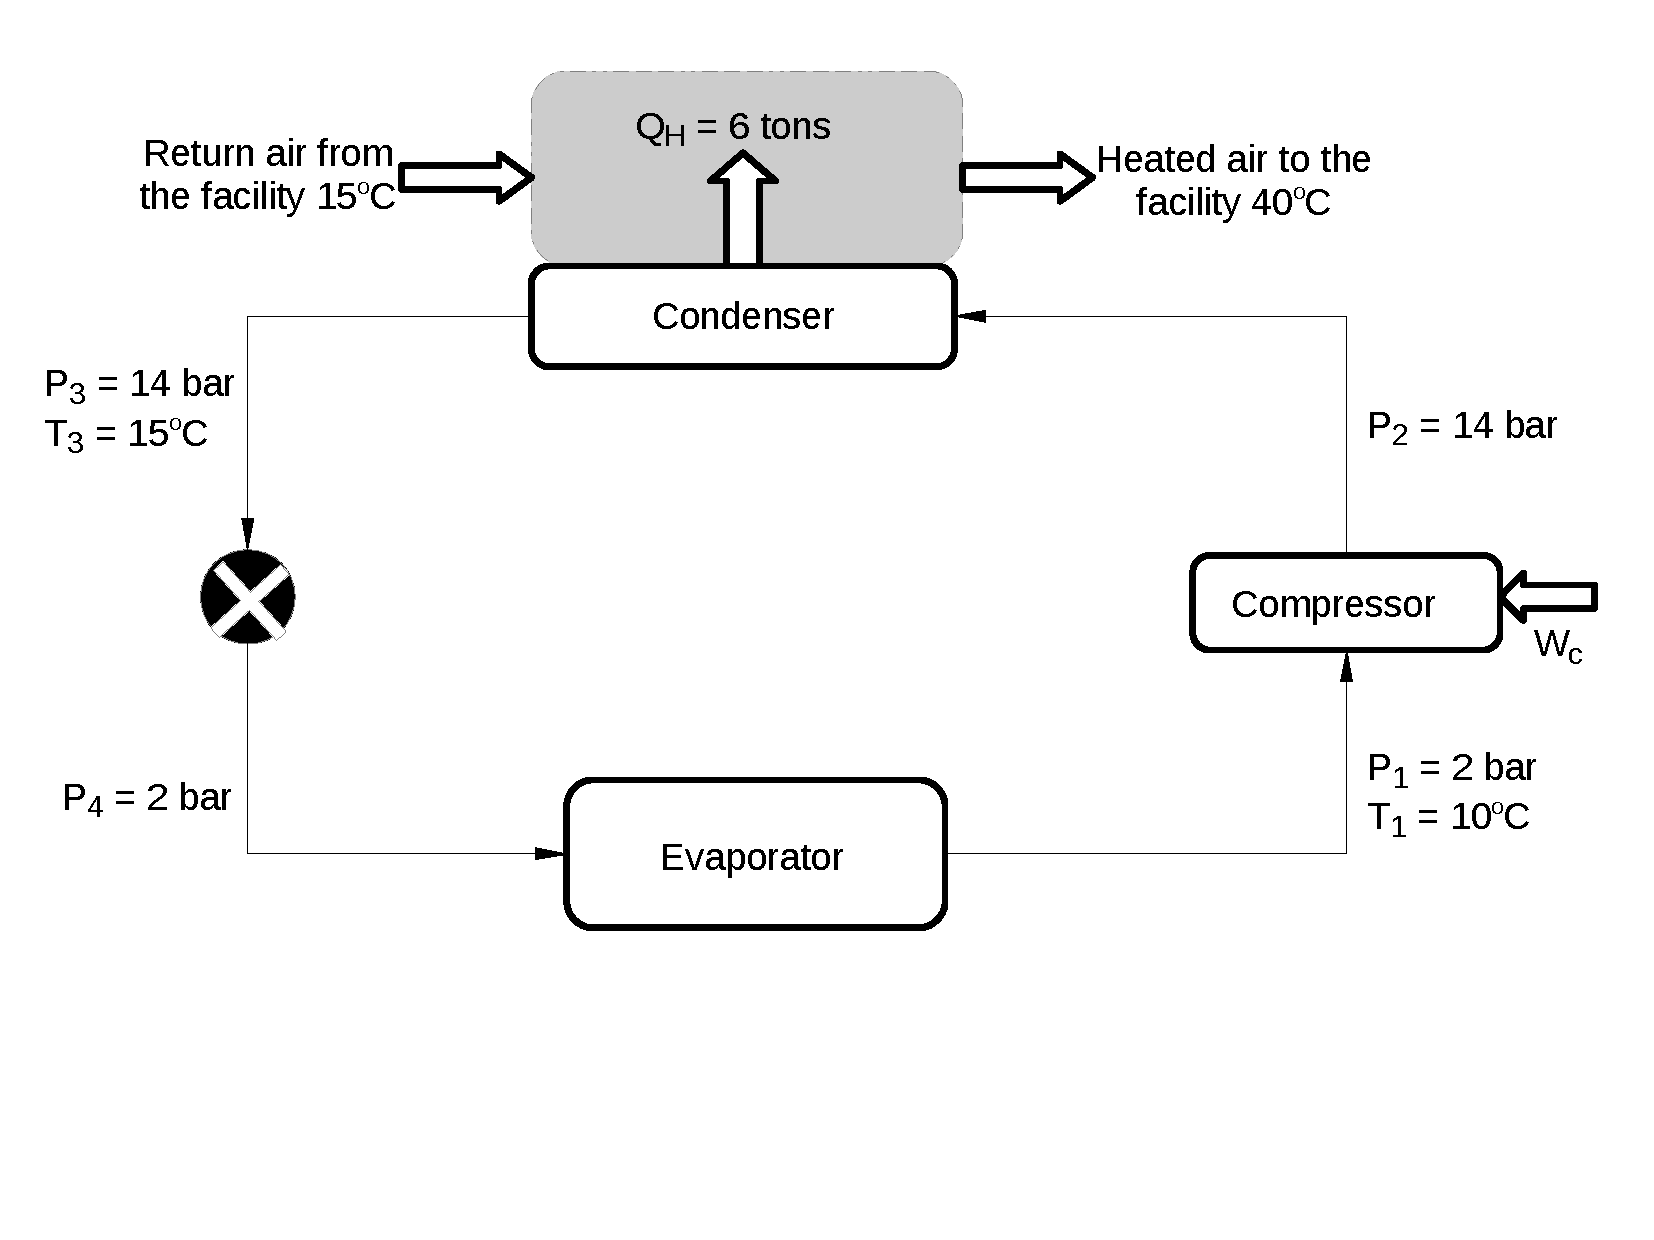
\includegraphics[width=16.0cm,height=12.0cm]{./Pics/Overview_Refrig42}
\end{center}
\caption{Heat pump cycle (Question 4).}\label{Exam01_Prob4}
\end{figure}


\end{question}

\clearpage


%%%
%%% Question 5
%%%
\begin{question}\vspace{-2\baselineskip}
\begin{enumerate}
%
\item A reciprocating engines was designed to operate with the following stages:
\begin{enumerate}
\item 1--2: Isentropic compression;
\item 2--3: Addition of heat at constant volume;
\item 3--4: Addition of heat at constant pressure;
\item 4--5: Isentropic expansion and;
\item 5--1: Rejection of heat at constant volume.
\end{enumerate}
Sketch the {\it TS} and {\it PV} diagrams for this cycle. {\bf[4 Marks]}
%
\item For this cycle, define an expression for the net work $\left(W_{\text{net}}\right)$ as a function of mass of air ($m$), heat capacities $\left(C_{p}\text{ and } C_{v}\right)$ and temperatures $\left(T_{j}\right)$, {\bf[6 Marks]}
\begin{displaymath}
W_{\text{net}}= W_{\text{net}}\left(m,C_{p},C_{v},T_{j}\right)=\text{Heat Supplied} - \text{Heat Rejected}
\end{displaymath}


%
\end{enumerate}

\end{question}



\vfill

\paperend

\end{document}
